%%%%%%%%%%%%%%%%%%%%%%%%%%%%%%%%%%%%%%%%%%%%%%%%%%%%%%%%%%%%%%%%%%%%%%%%%%%%%%%%%
%% Document: Thesis for PhD at UC Riverside                                    %%
%% Title: Investigating the evolution of environmental and biotic interactions %%
%%          in basal fungal lineages through comparative genomics              %%
%% Author: Steven Ahrendt                                                      %%
%%%%%%%%%%%%%%%%%%%%%%%%%%%%%%%%%%%%%%%%%%%%%%%%%%%%%%%%%%%%%%%%%%%%%%%%%%%%%%%%%
%% COELOMOMYCES FIGURES %%
%%%%%%%%%%%%%%%%%%%%%%%%%%
% GO-slim plot
\begin{figure}[tbp]
  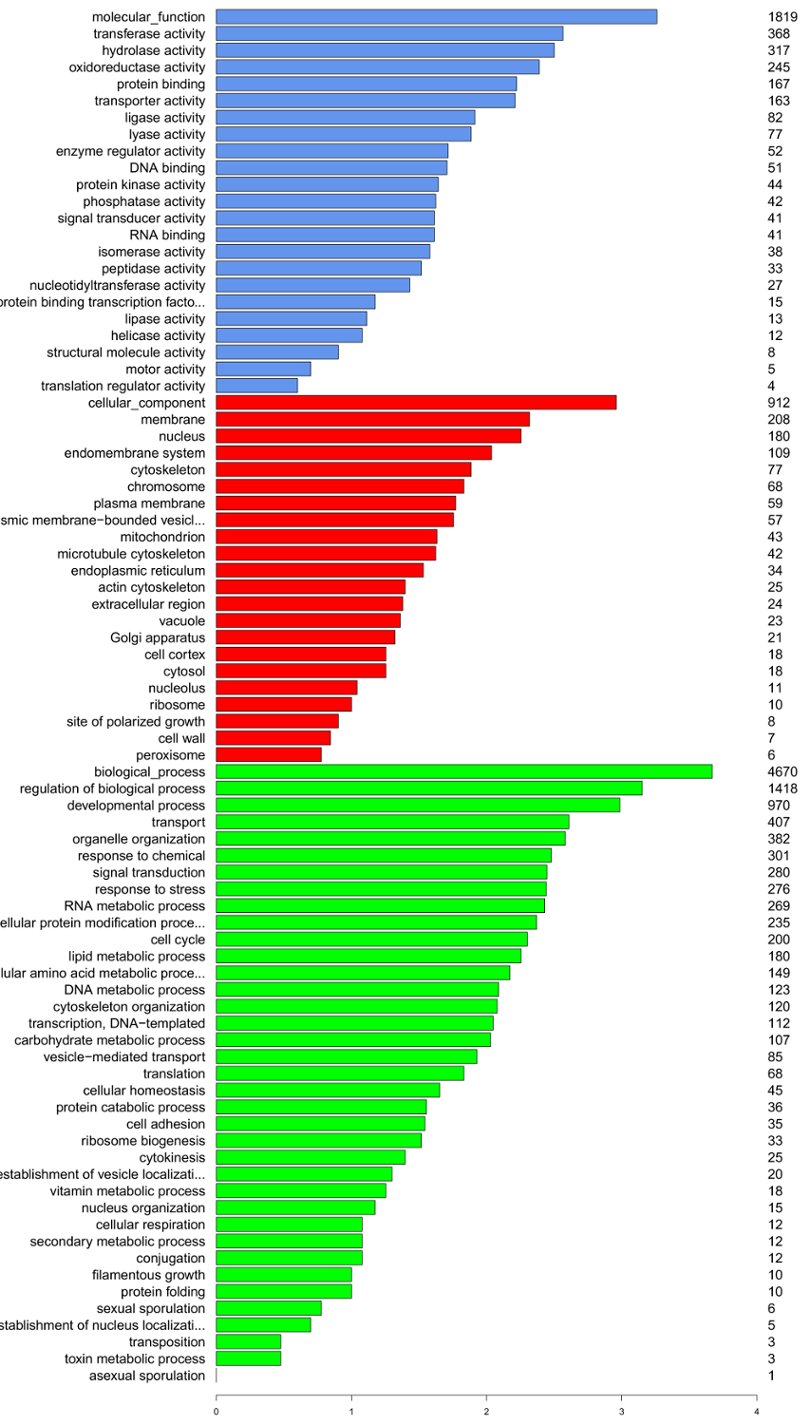
\includegraphics[width=4in]{./Chapter_Coelomomyces/img/Clat_aspergillus_GOPlot.png}
  \caption[\textit{C. lat} transcriptome GO term distribution]{Horizontal bar chart showing the distribution of \textit{Aspergillus} GO-Slim terms associated with the \textit{C. lativitattus} transcriptome. X axis is a logarithmic scale.}
  \label{fig:ChClat_GOPlot}
\end{figure}

% Opsin-GC fusion; chytrid cluster
\begin{figure}[tbp]
  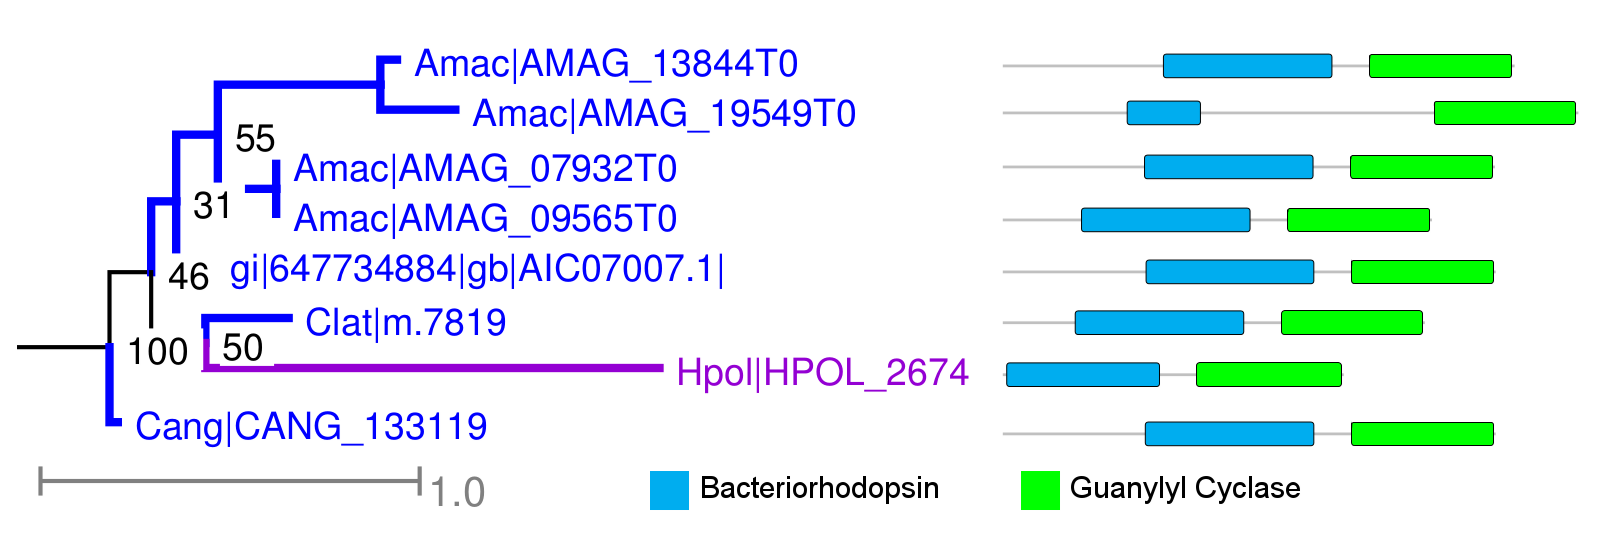
\includegraphics[width=4in]{./Chapter_Coelomomyces/img/OpsinGCFusion_chytridCluster.png}
  \caption[Opsin-GC fusion proteins]{A subset of bacterial opsin-guanylate cyclase fusion proteins. Proteins with similar architecture as described for \textit{B. emersonii} identified in Blastocladiomycete and Chytridiomycete proteomes, and \textit{C. lativitattus} transcriptome.}
  \label{fig:ChClat_OpsinGCFusion}
\end{figure}
\hfill \break
% Beta-carotene distribution
\begin{figure}[tbp]
  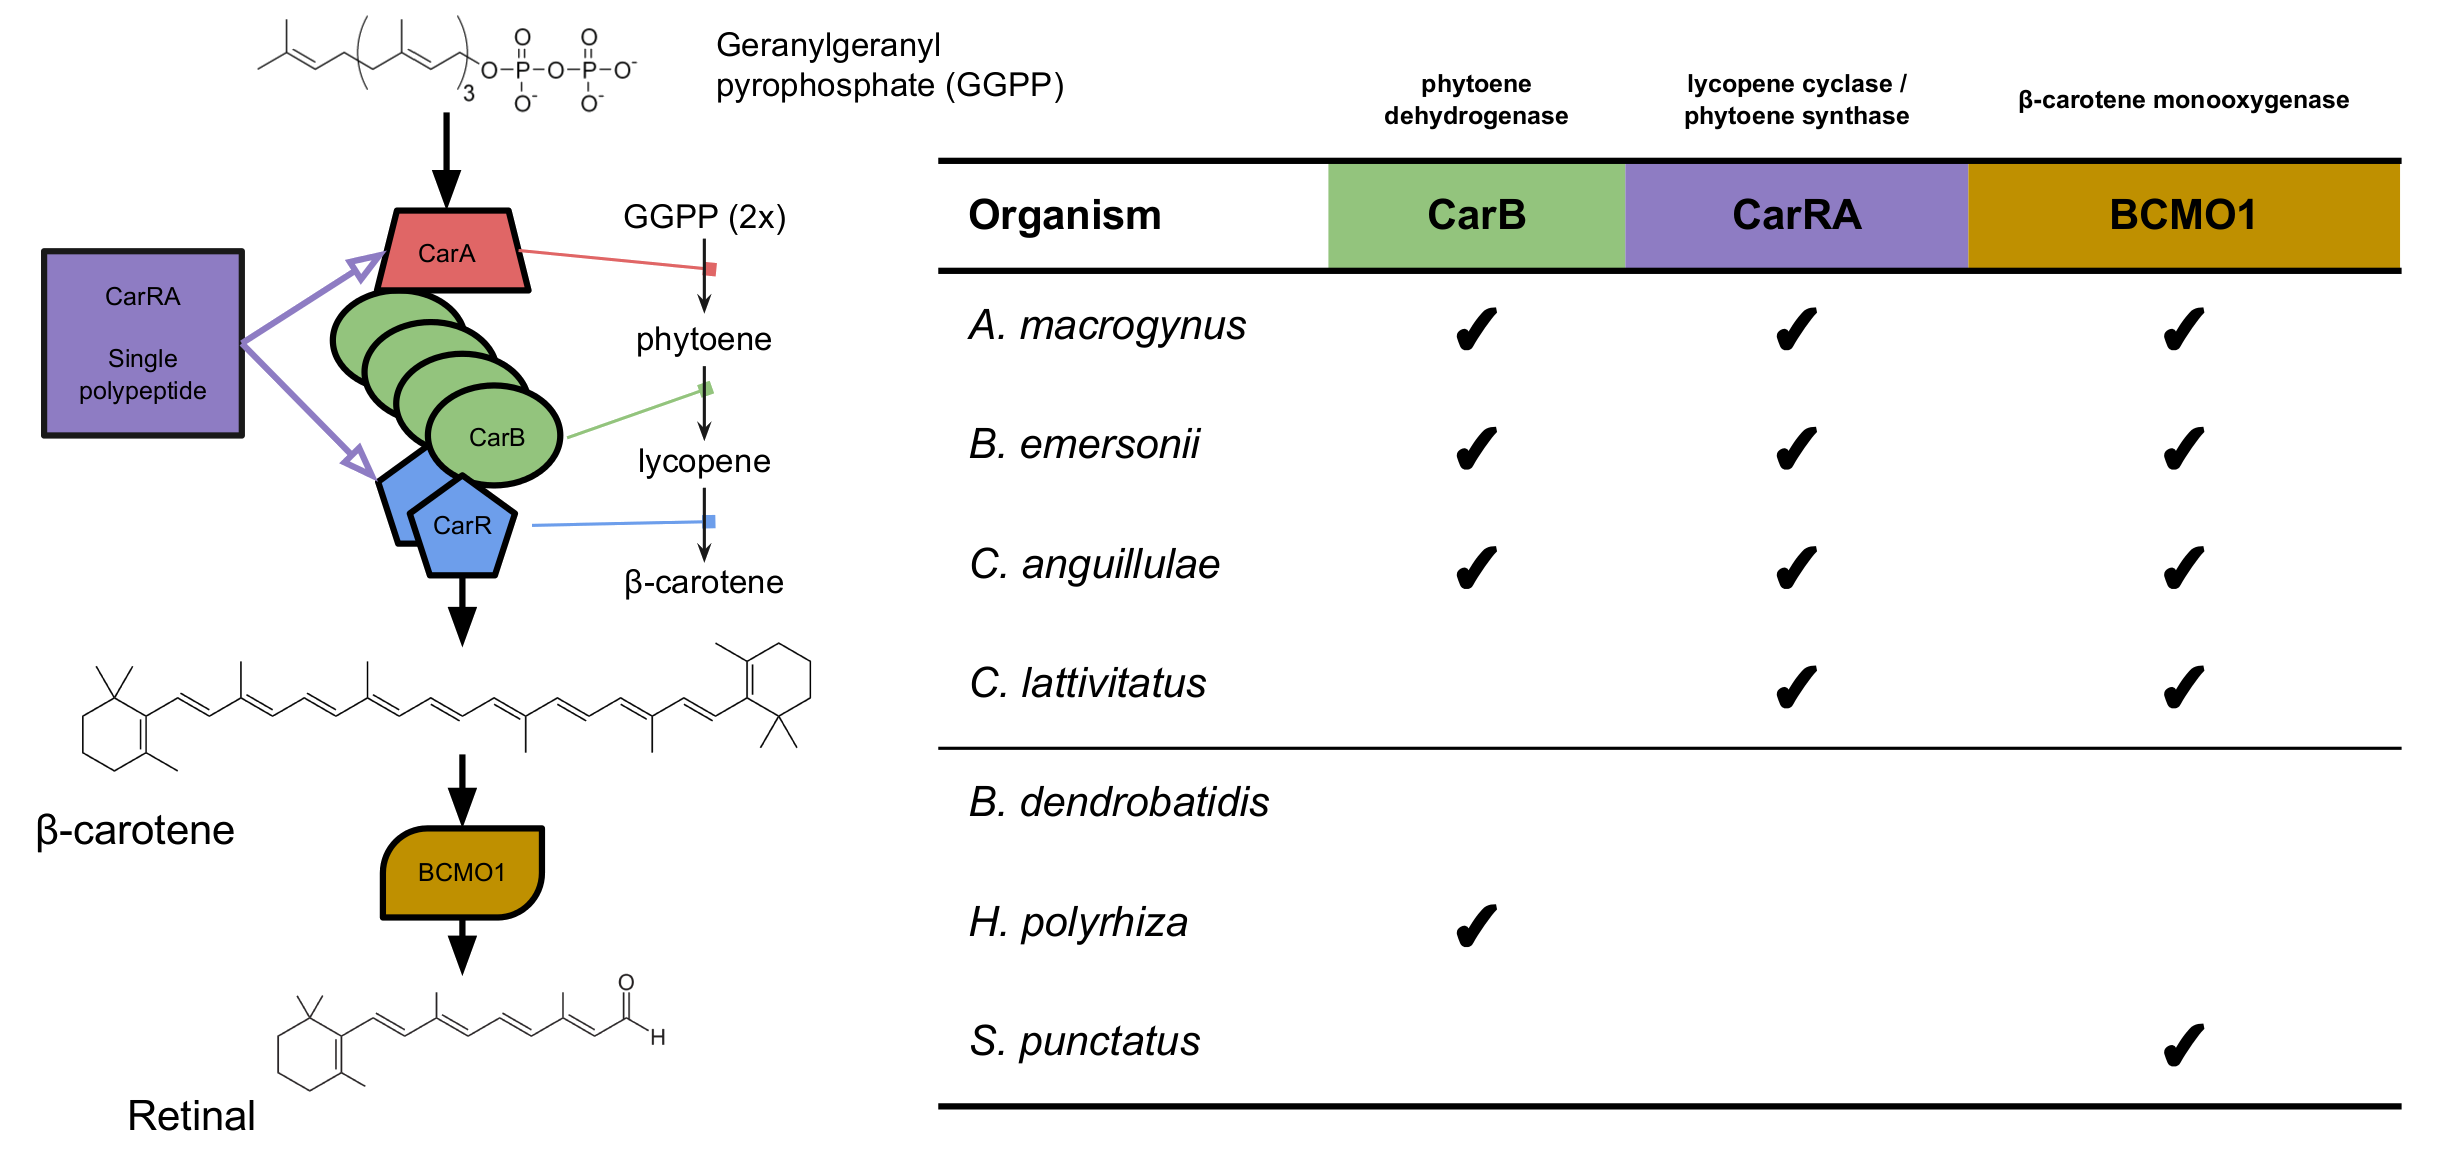
\includegraphics[width=4in]{./Chapter_Coelomomyces/img/Figure_bcaroPresenceAbsence.png}
  \caption[$\beta$-carotene enzyme presence / absence]{Presence and absence of $\beta$-carotene related proteins in species belonging to the Chytridiomycota and Blastocladiomycota.}
  \label{fig:ChClat_Bcaro}
\end{figure}

% PF00112 tree
\begin{figure}[tbp]
  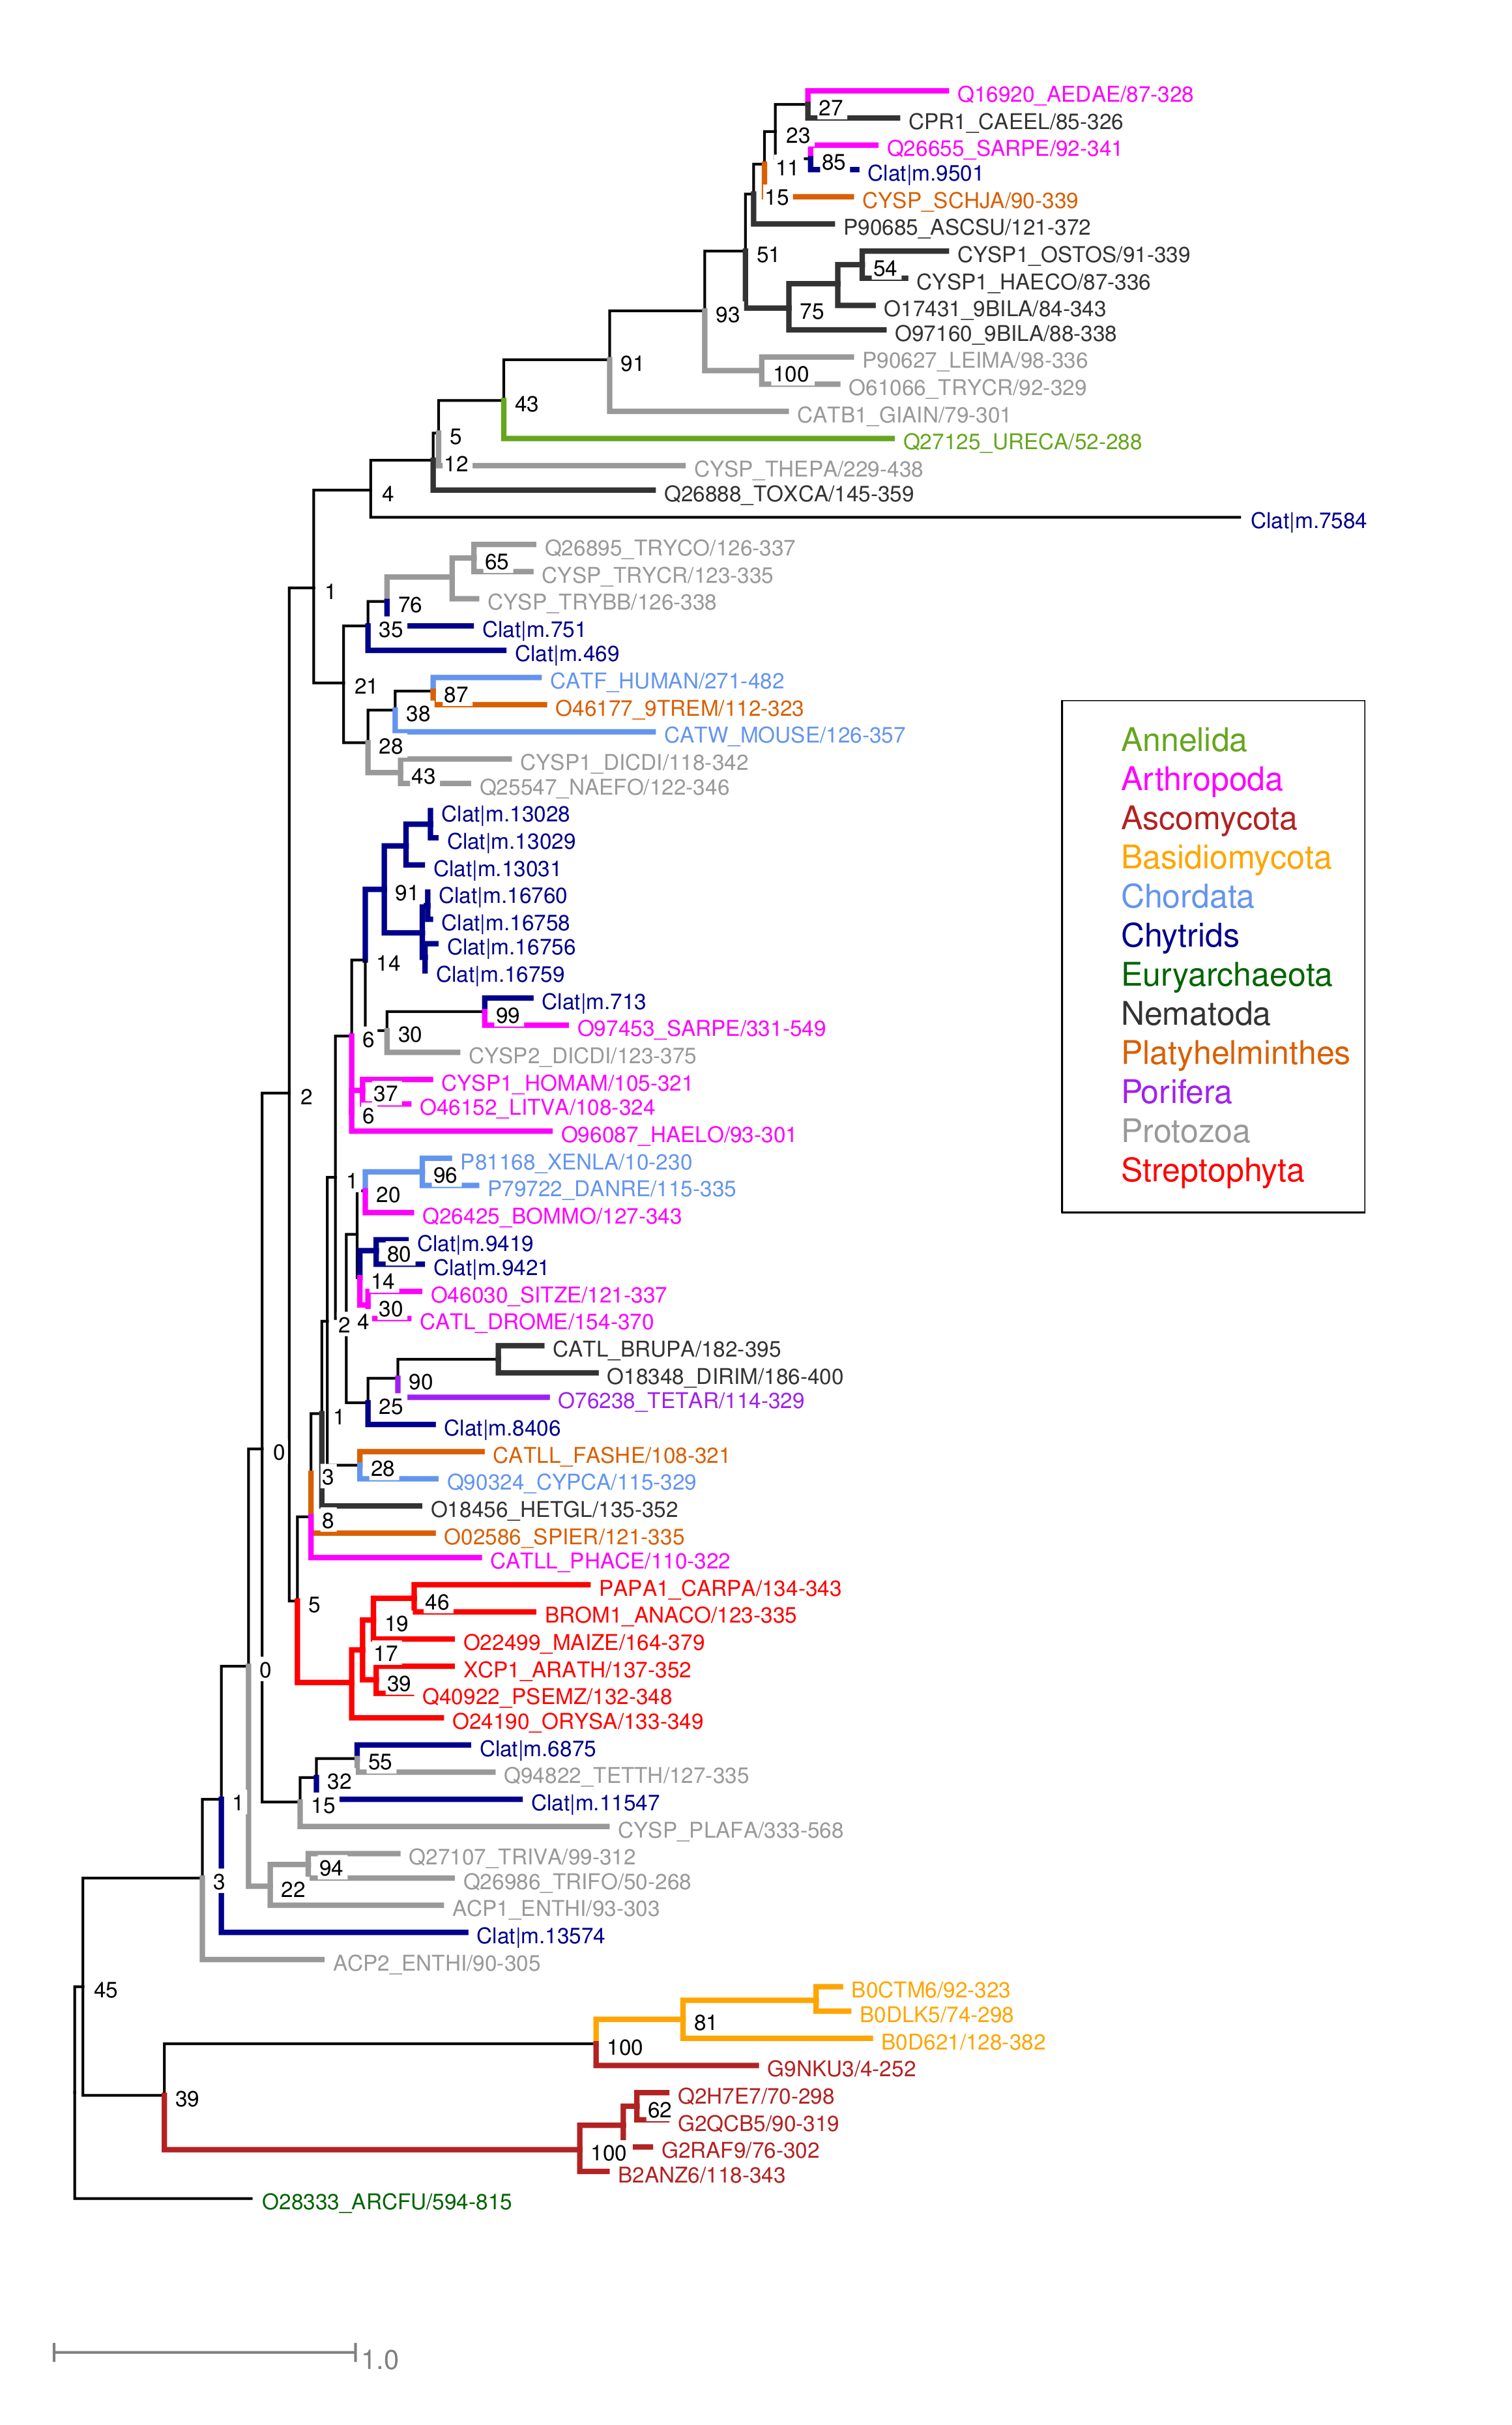
\includegraphics[width=4in]{./Chapter_Coelomomyces/img/PF00112_tree.png}
  \caption[PF00112 RAxML tree]{RAxML tree of select PF00112 seed sequences, unique \textit{C. lat} protein sequences, and sequences from Dikarya species.}
  \label{fig:ChClat_PF00112}
\end{figure}

% PF00089 tree
\begin{figure}[tbp]
  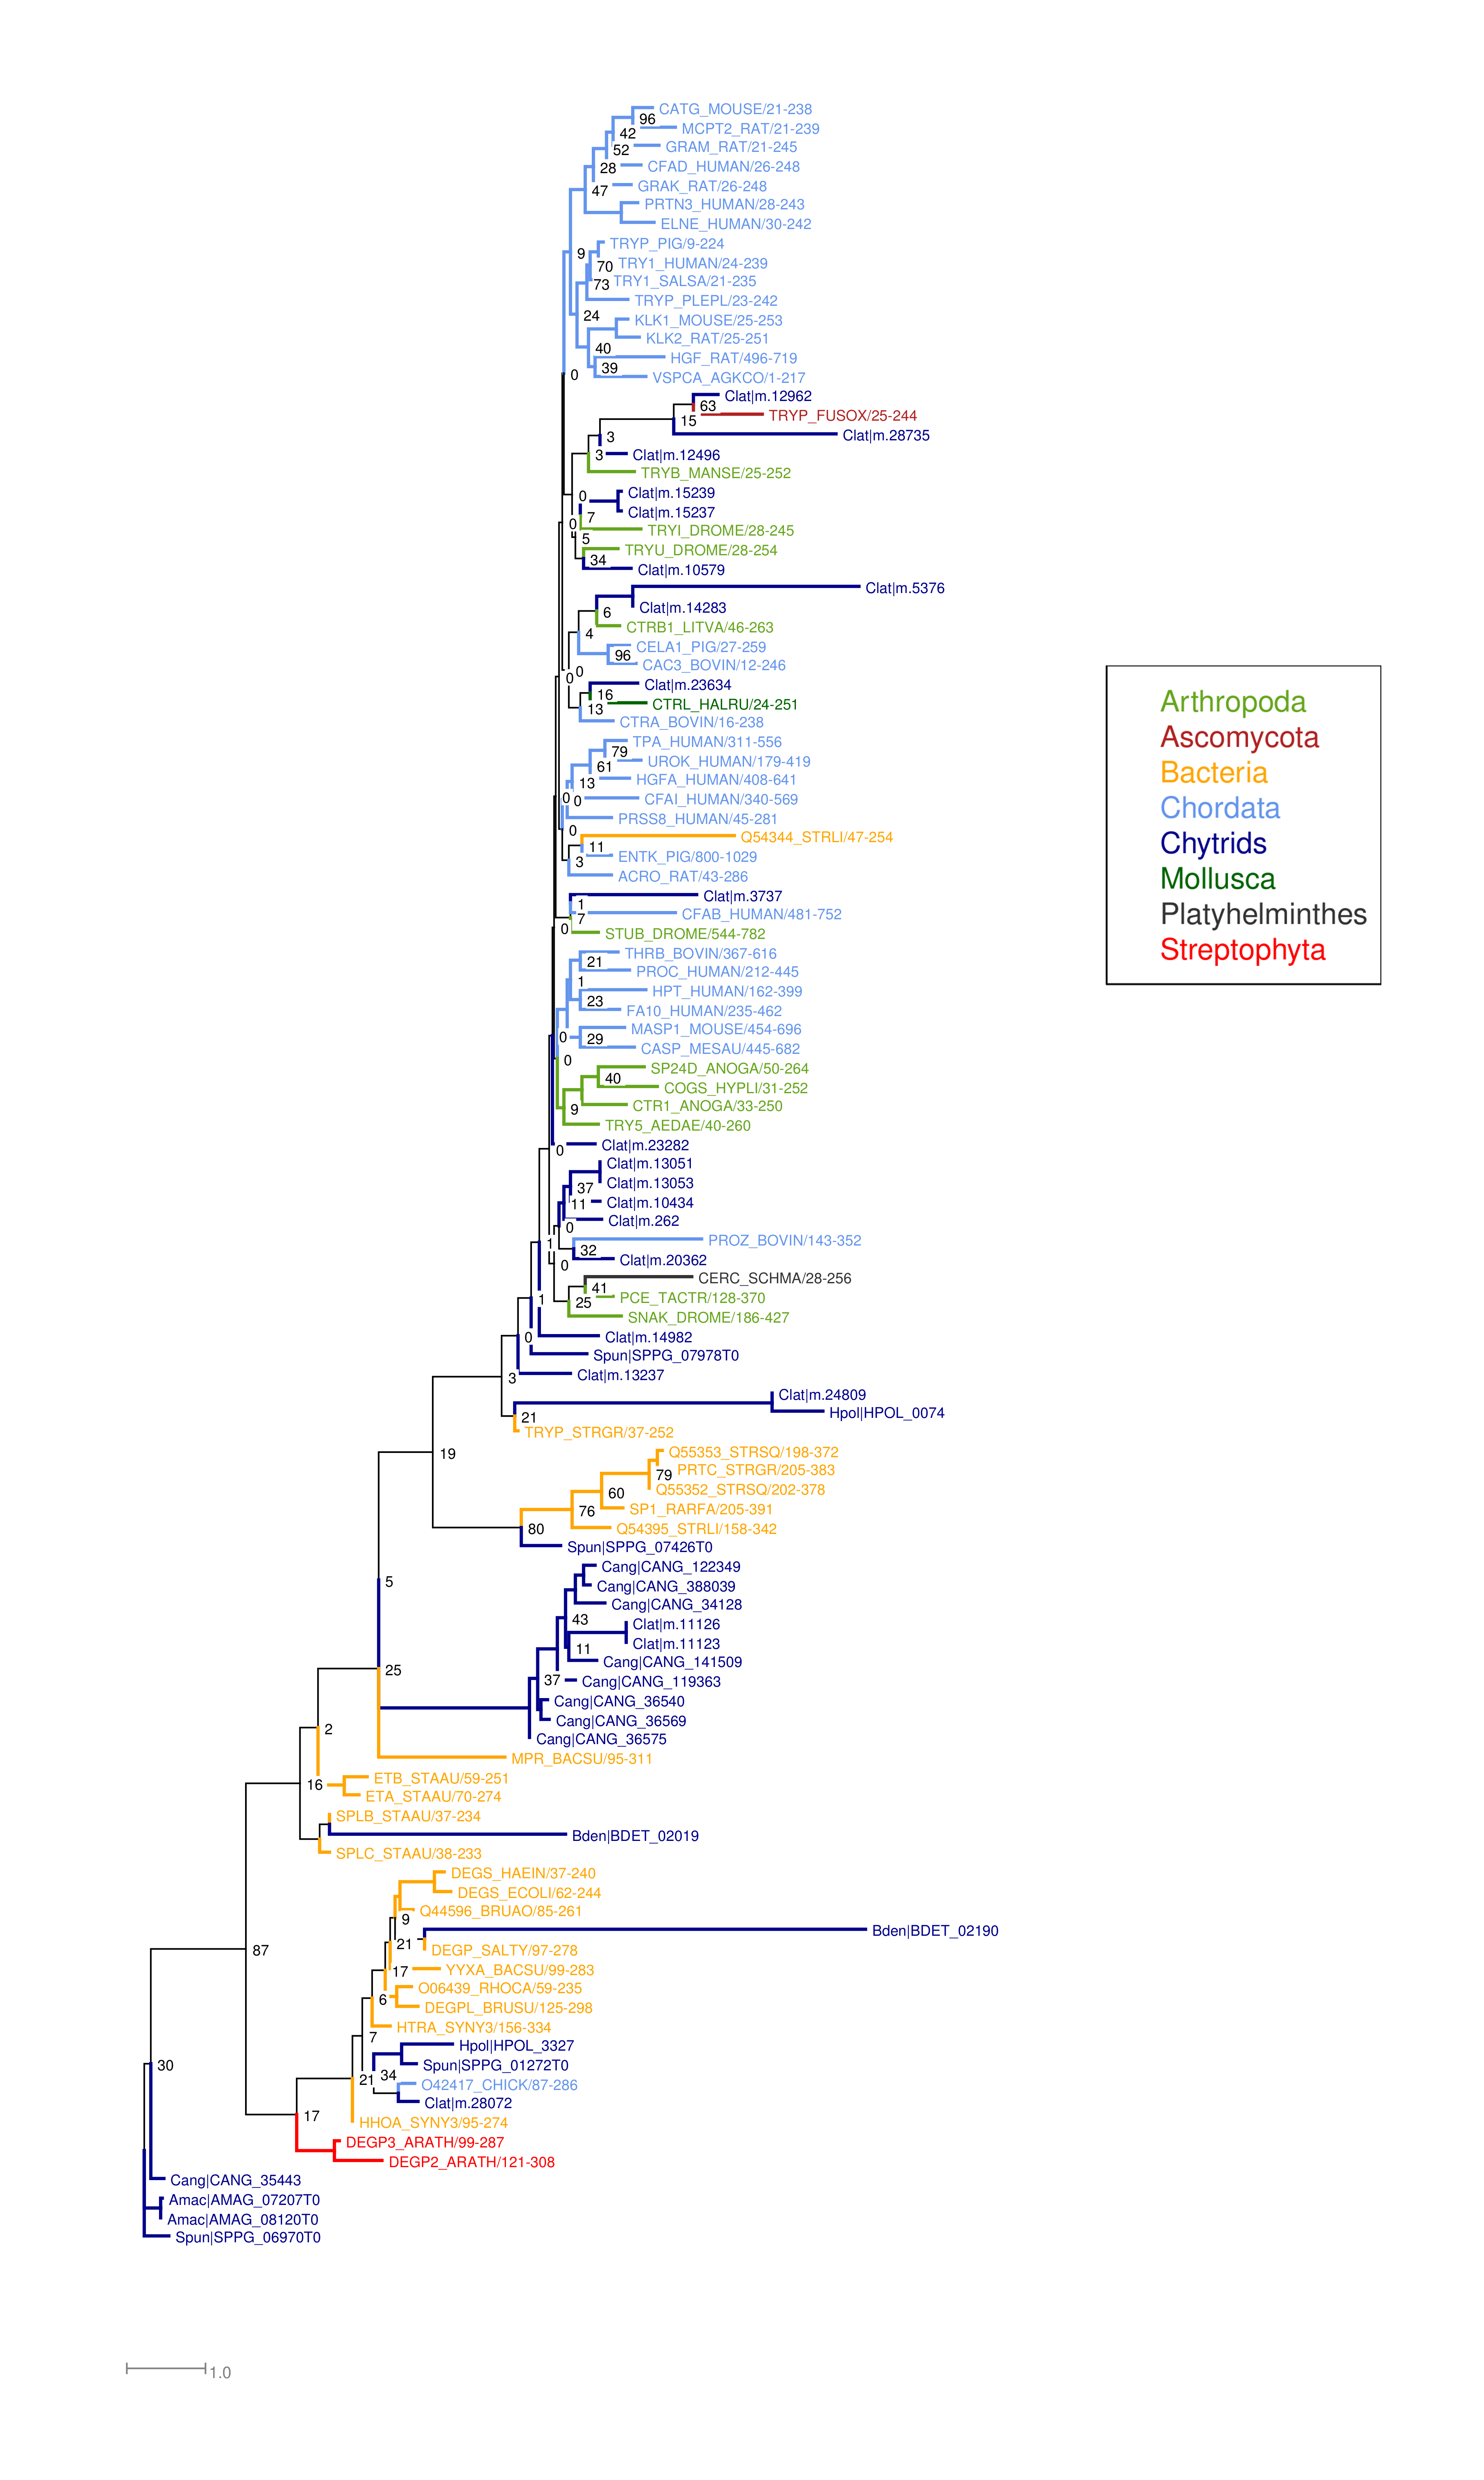
\includegraphics[width=4in]{./Chapter_Coelomomyces/img/PF00089_tree.png}
  \caption[PF00089 RAxML tree]{RAxML tree of select PF0089 seed sequences and unique \textit{C. lat} protein sequences}
  \label{fig:ChClat_PF00089}
\end{figure}

% 20HE receptor alignment
\begin{figure}[tbp]
  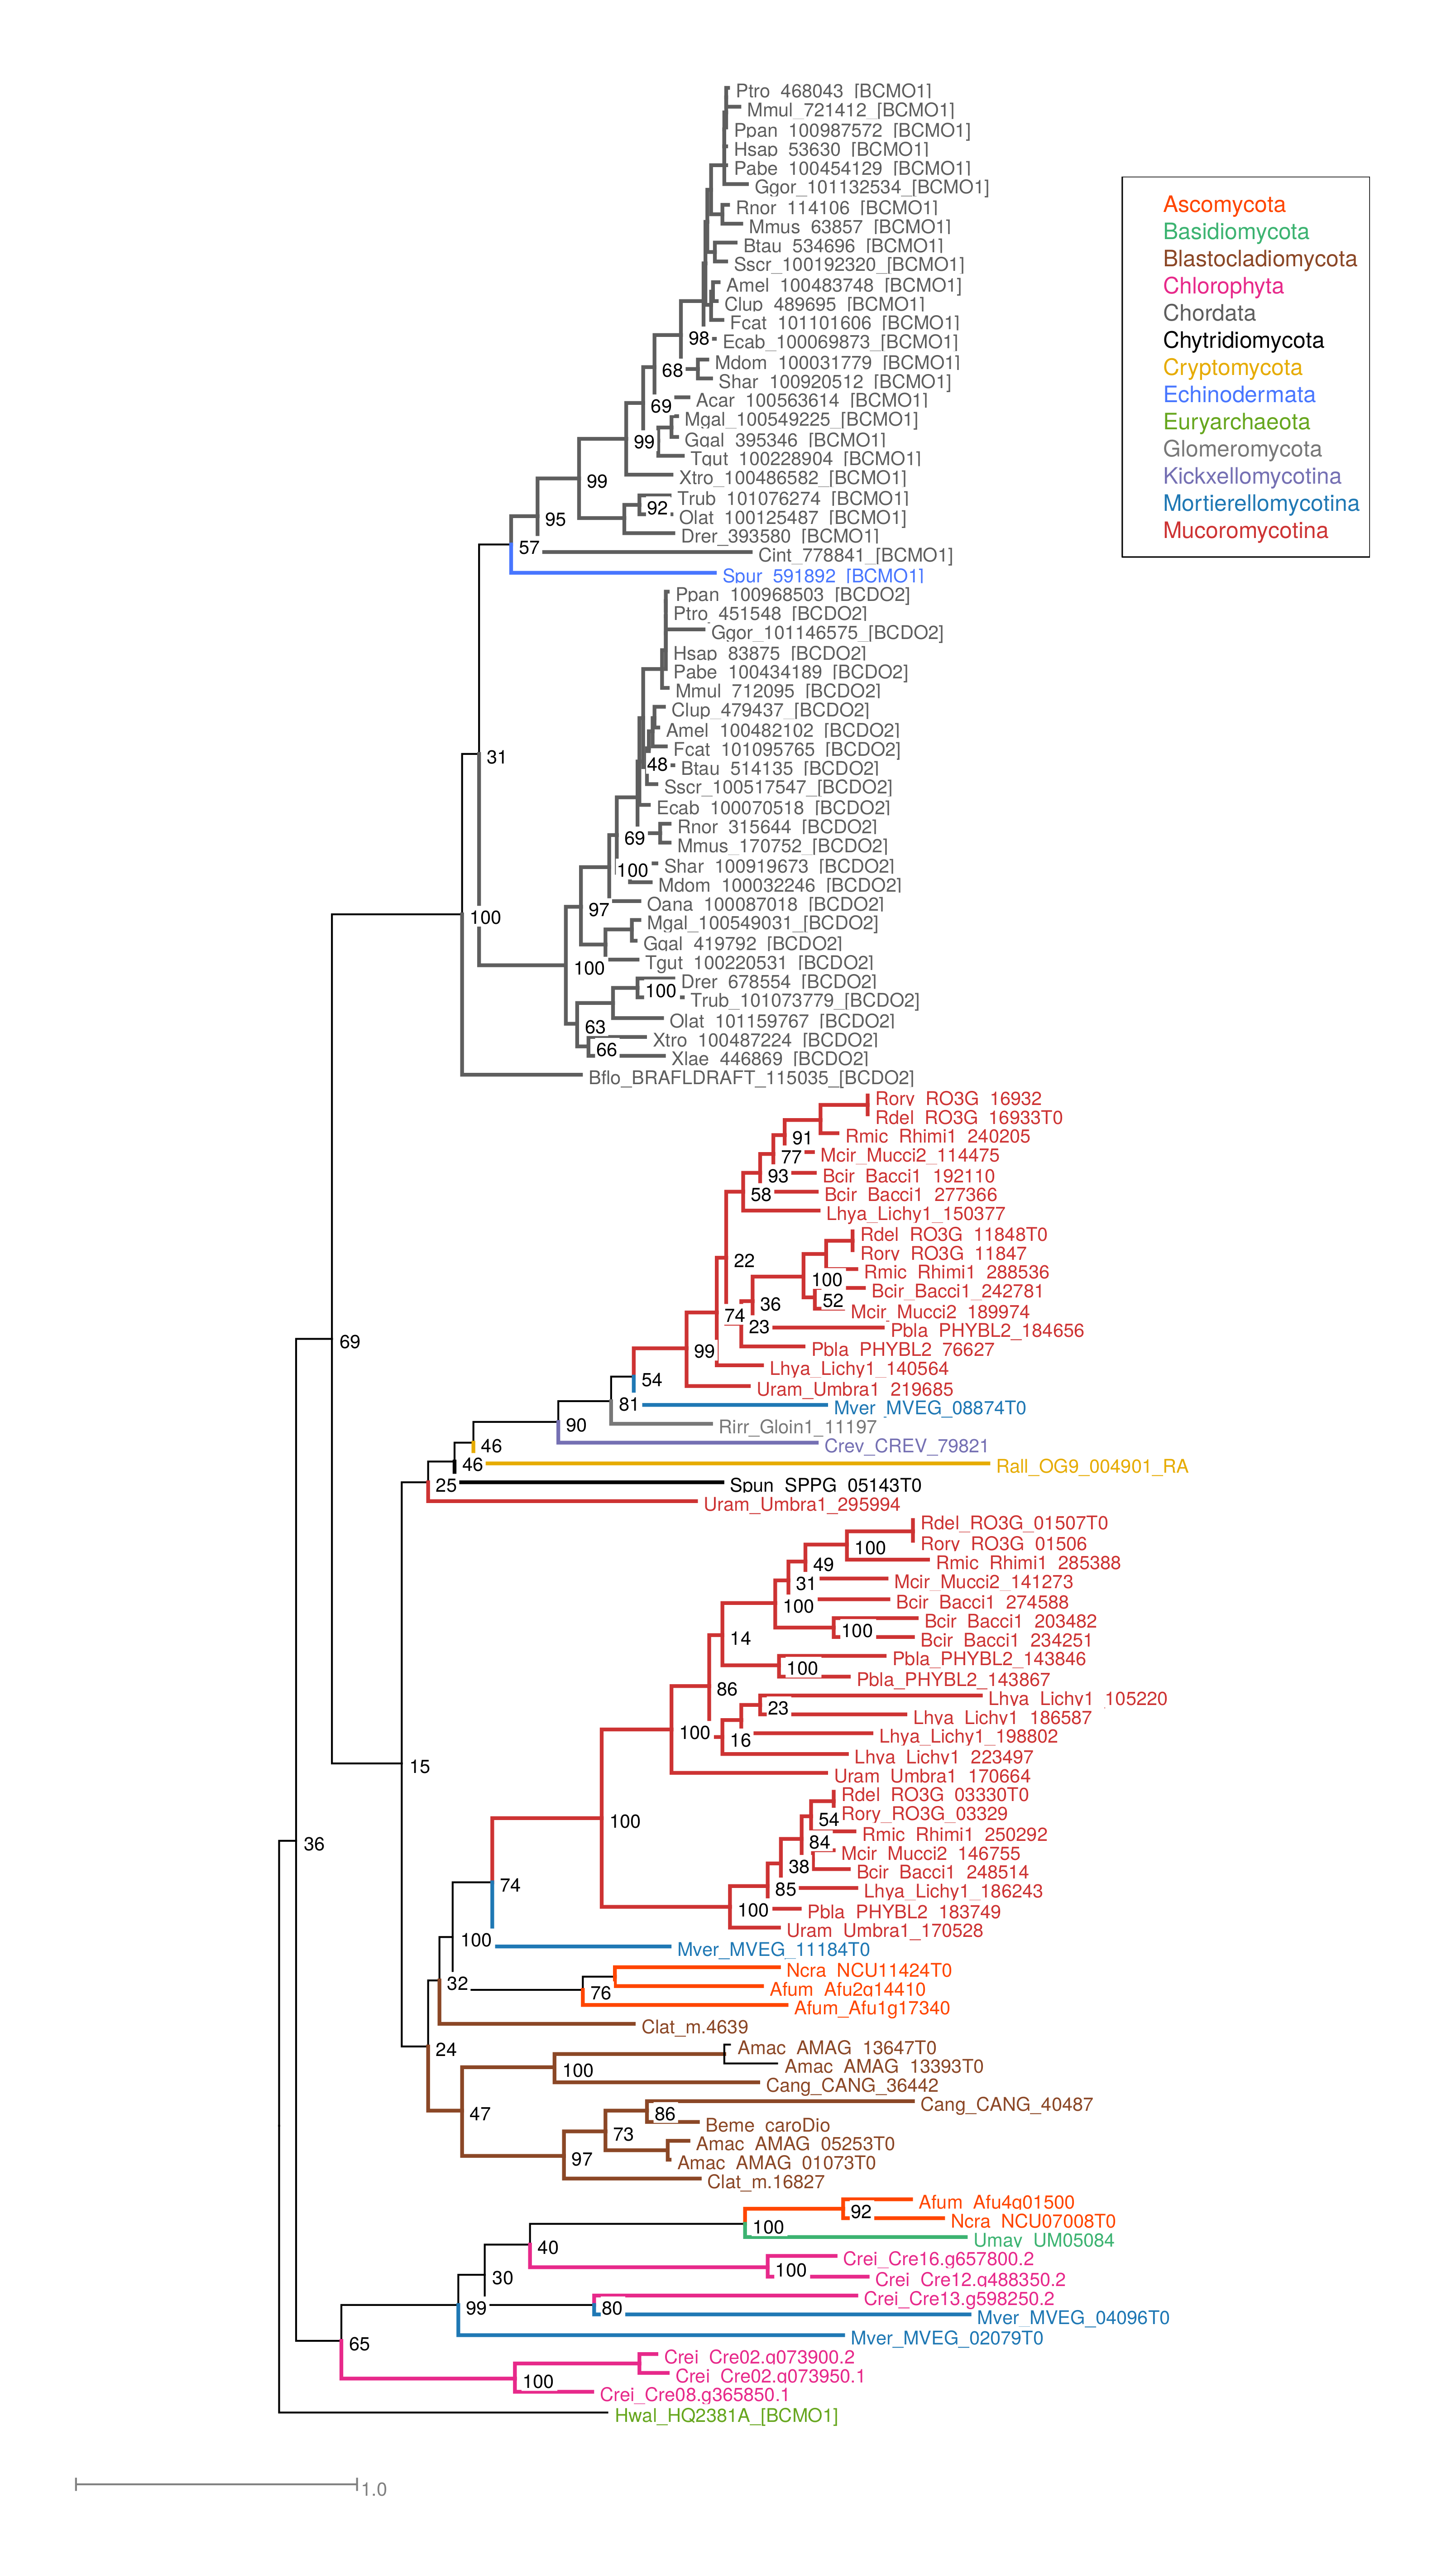
\includegraphics[width=4in]{./Chapter_Coelomomyces/img/BCMO1DO2.png}
%  \begin{texshade}{./Chapter_Coelomomyces/dat/20HE_alignment.fa_aln}
%    \threshold[80]{50}
%    \shadingmode[allmatchspecial]{similar}
%    \setends{1}{1..300}
%    \hideconsensus
%  \end{texshade}
  \caption[20HE alignment]{Alignment of \textit{D. melanogaster} EcR and putative 20HE receptors identified in \textit{C. lativittatus} }
  \label{fig:ChClat_20HEalign}
\end{figure}

% 20HE RAxML tree
\begin{figure}[tbp]
  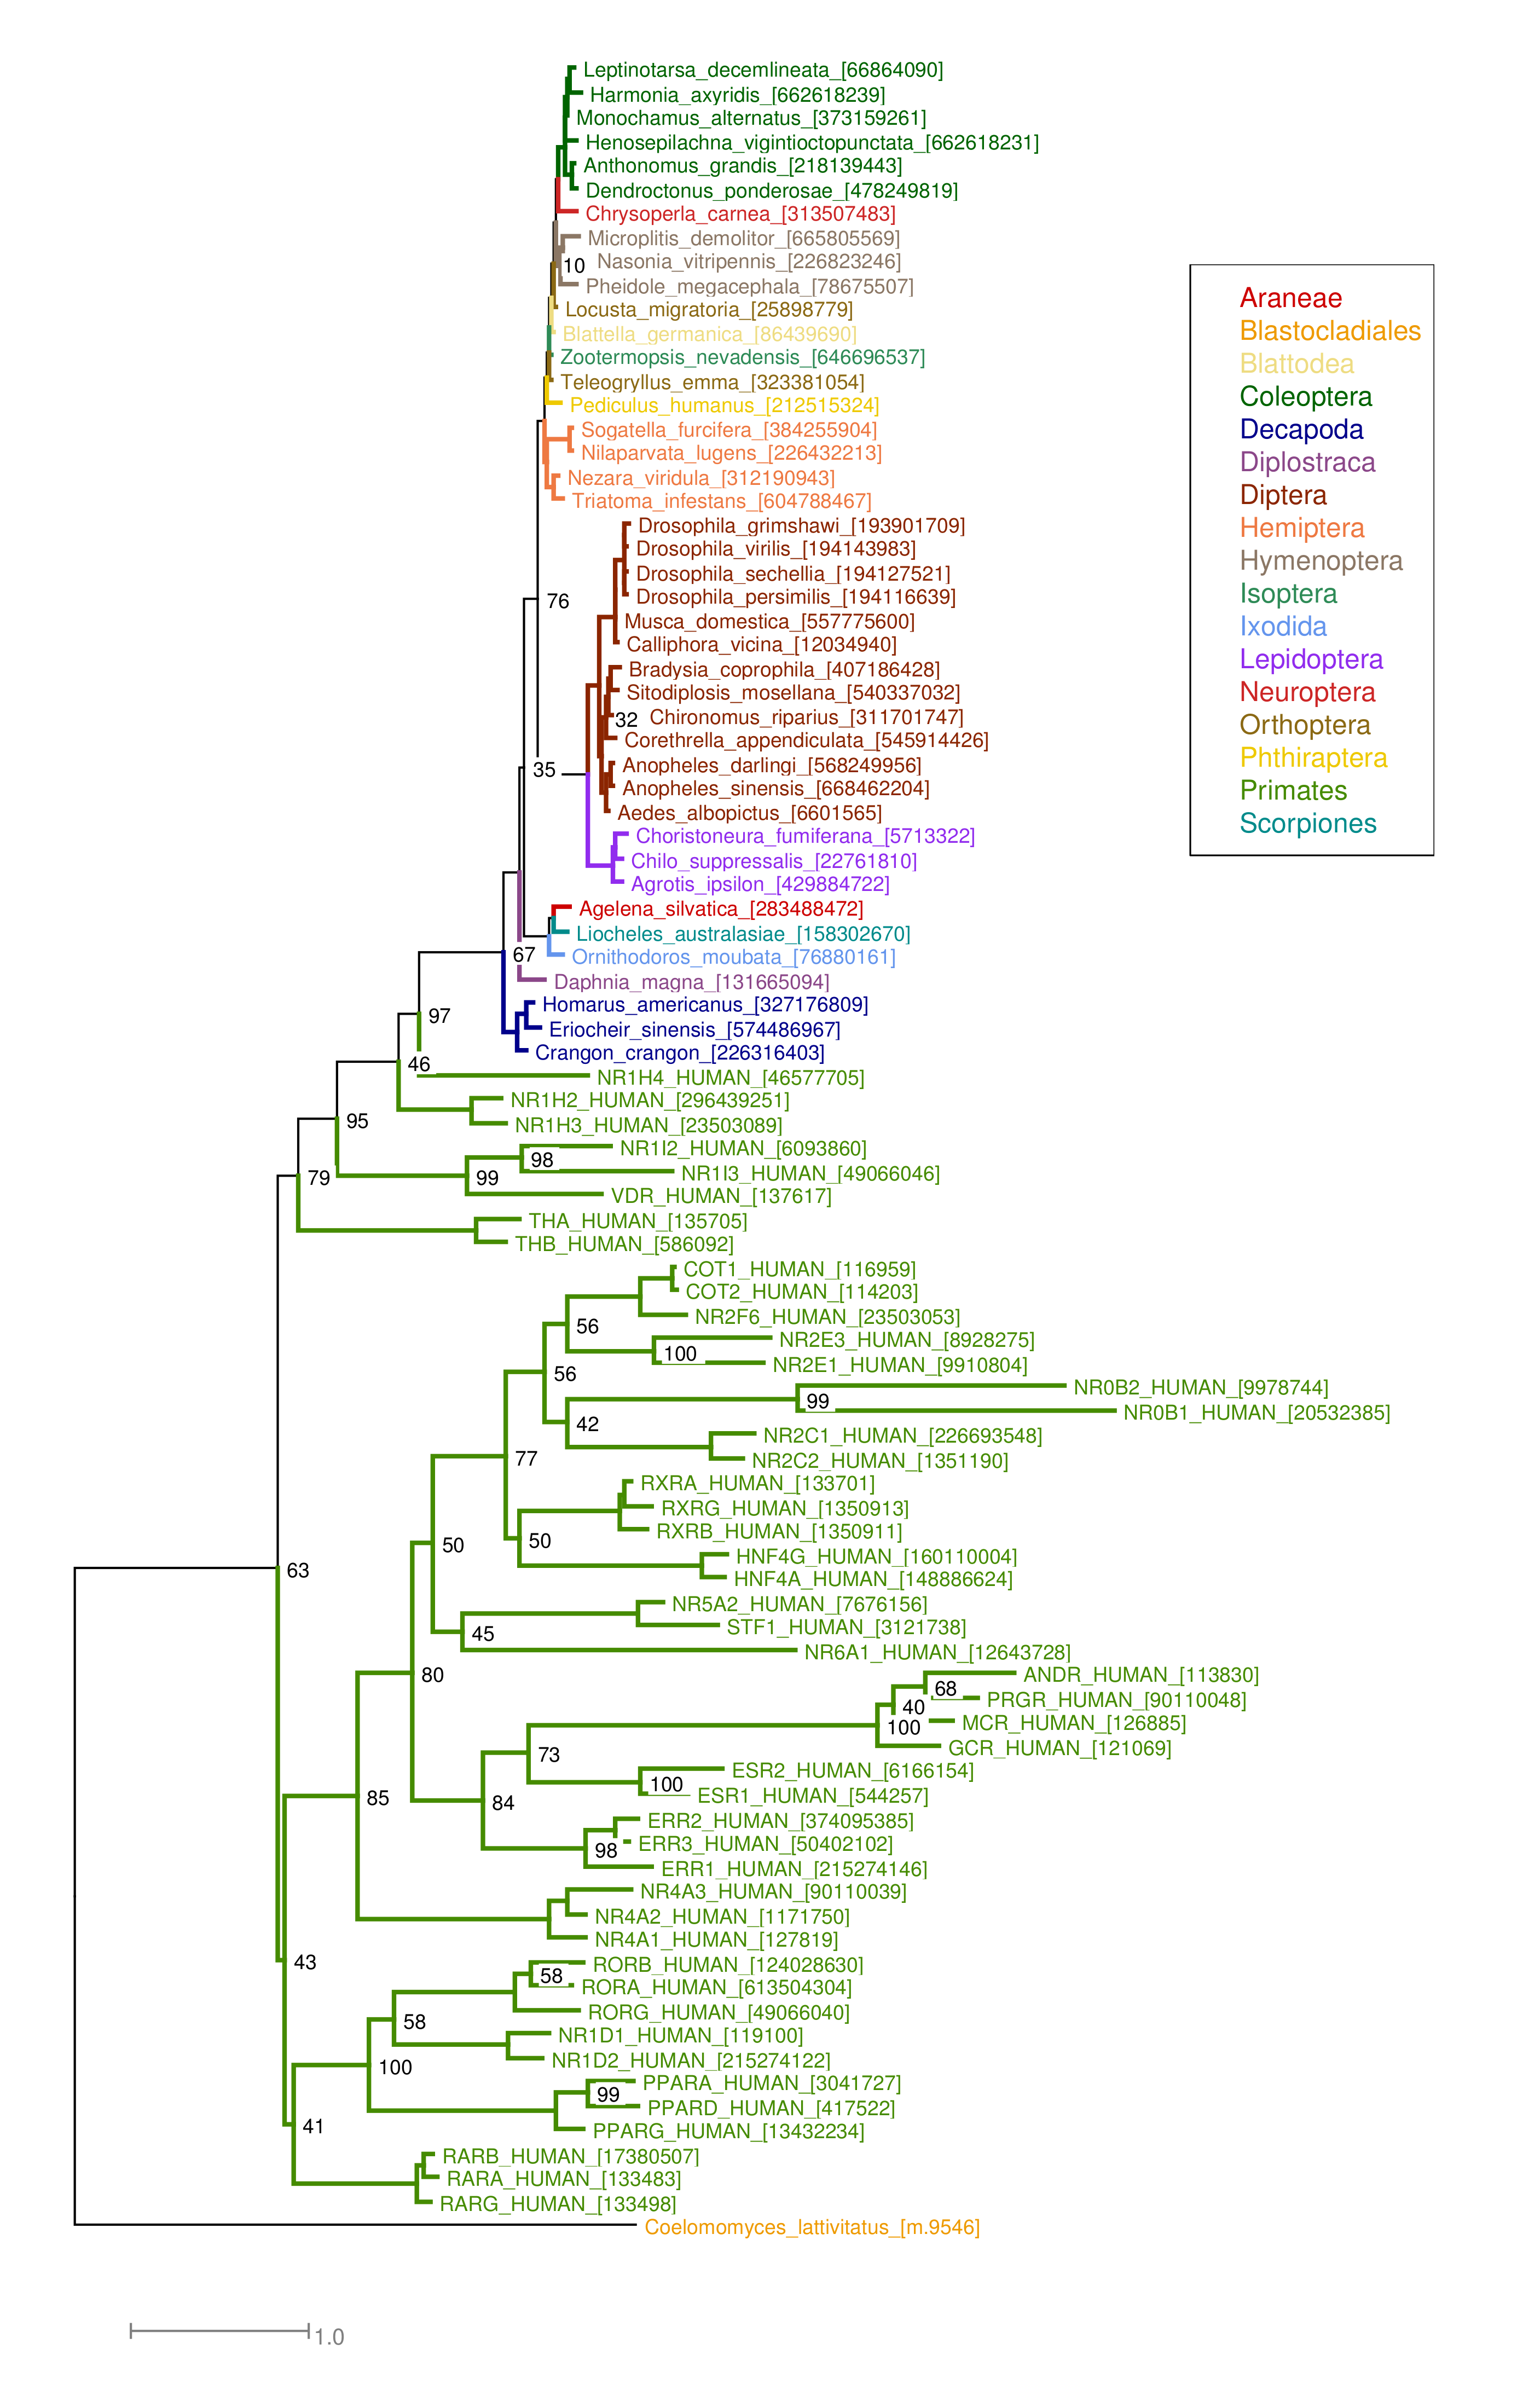
\includegraphics[width=4in]{./Chapter_Coelomomyces/img/20HE_NR_RAxMLTree.png}
  \caption[20HE and Nuclear Receptor RAxML tree]{RAxML tree of select 20-hydroxyecdysone receptors from insects and Human nuclear receptors, and unique \textit{C. lat} protein sequences}
  \label{fig:ChClat_20HE_NRtree}
\end{figure}

% BCMO1DO2 tree
\begin{figure}[tbp]
  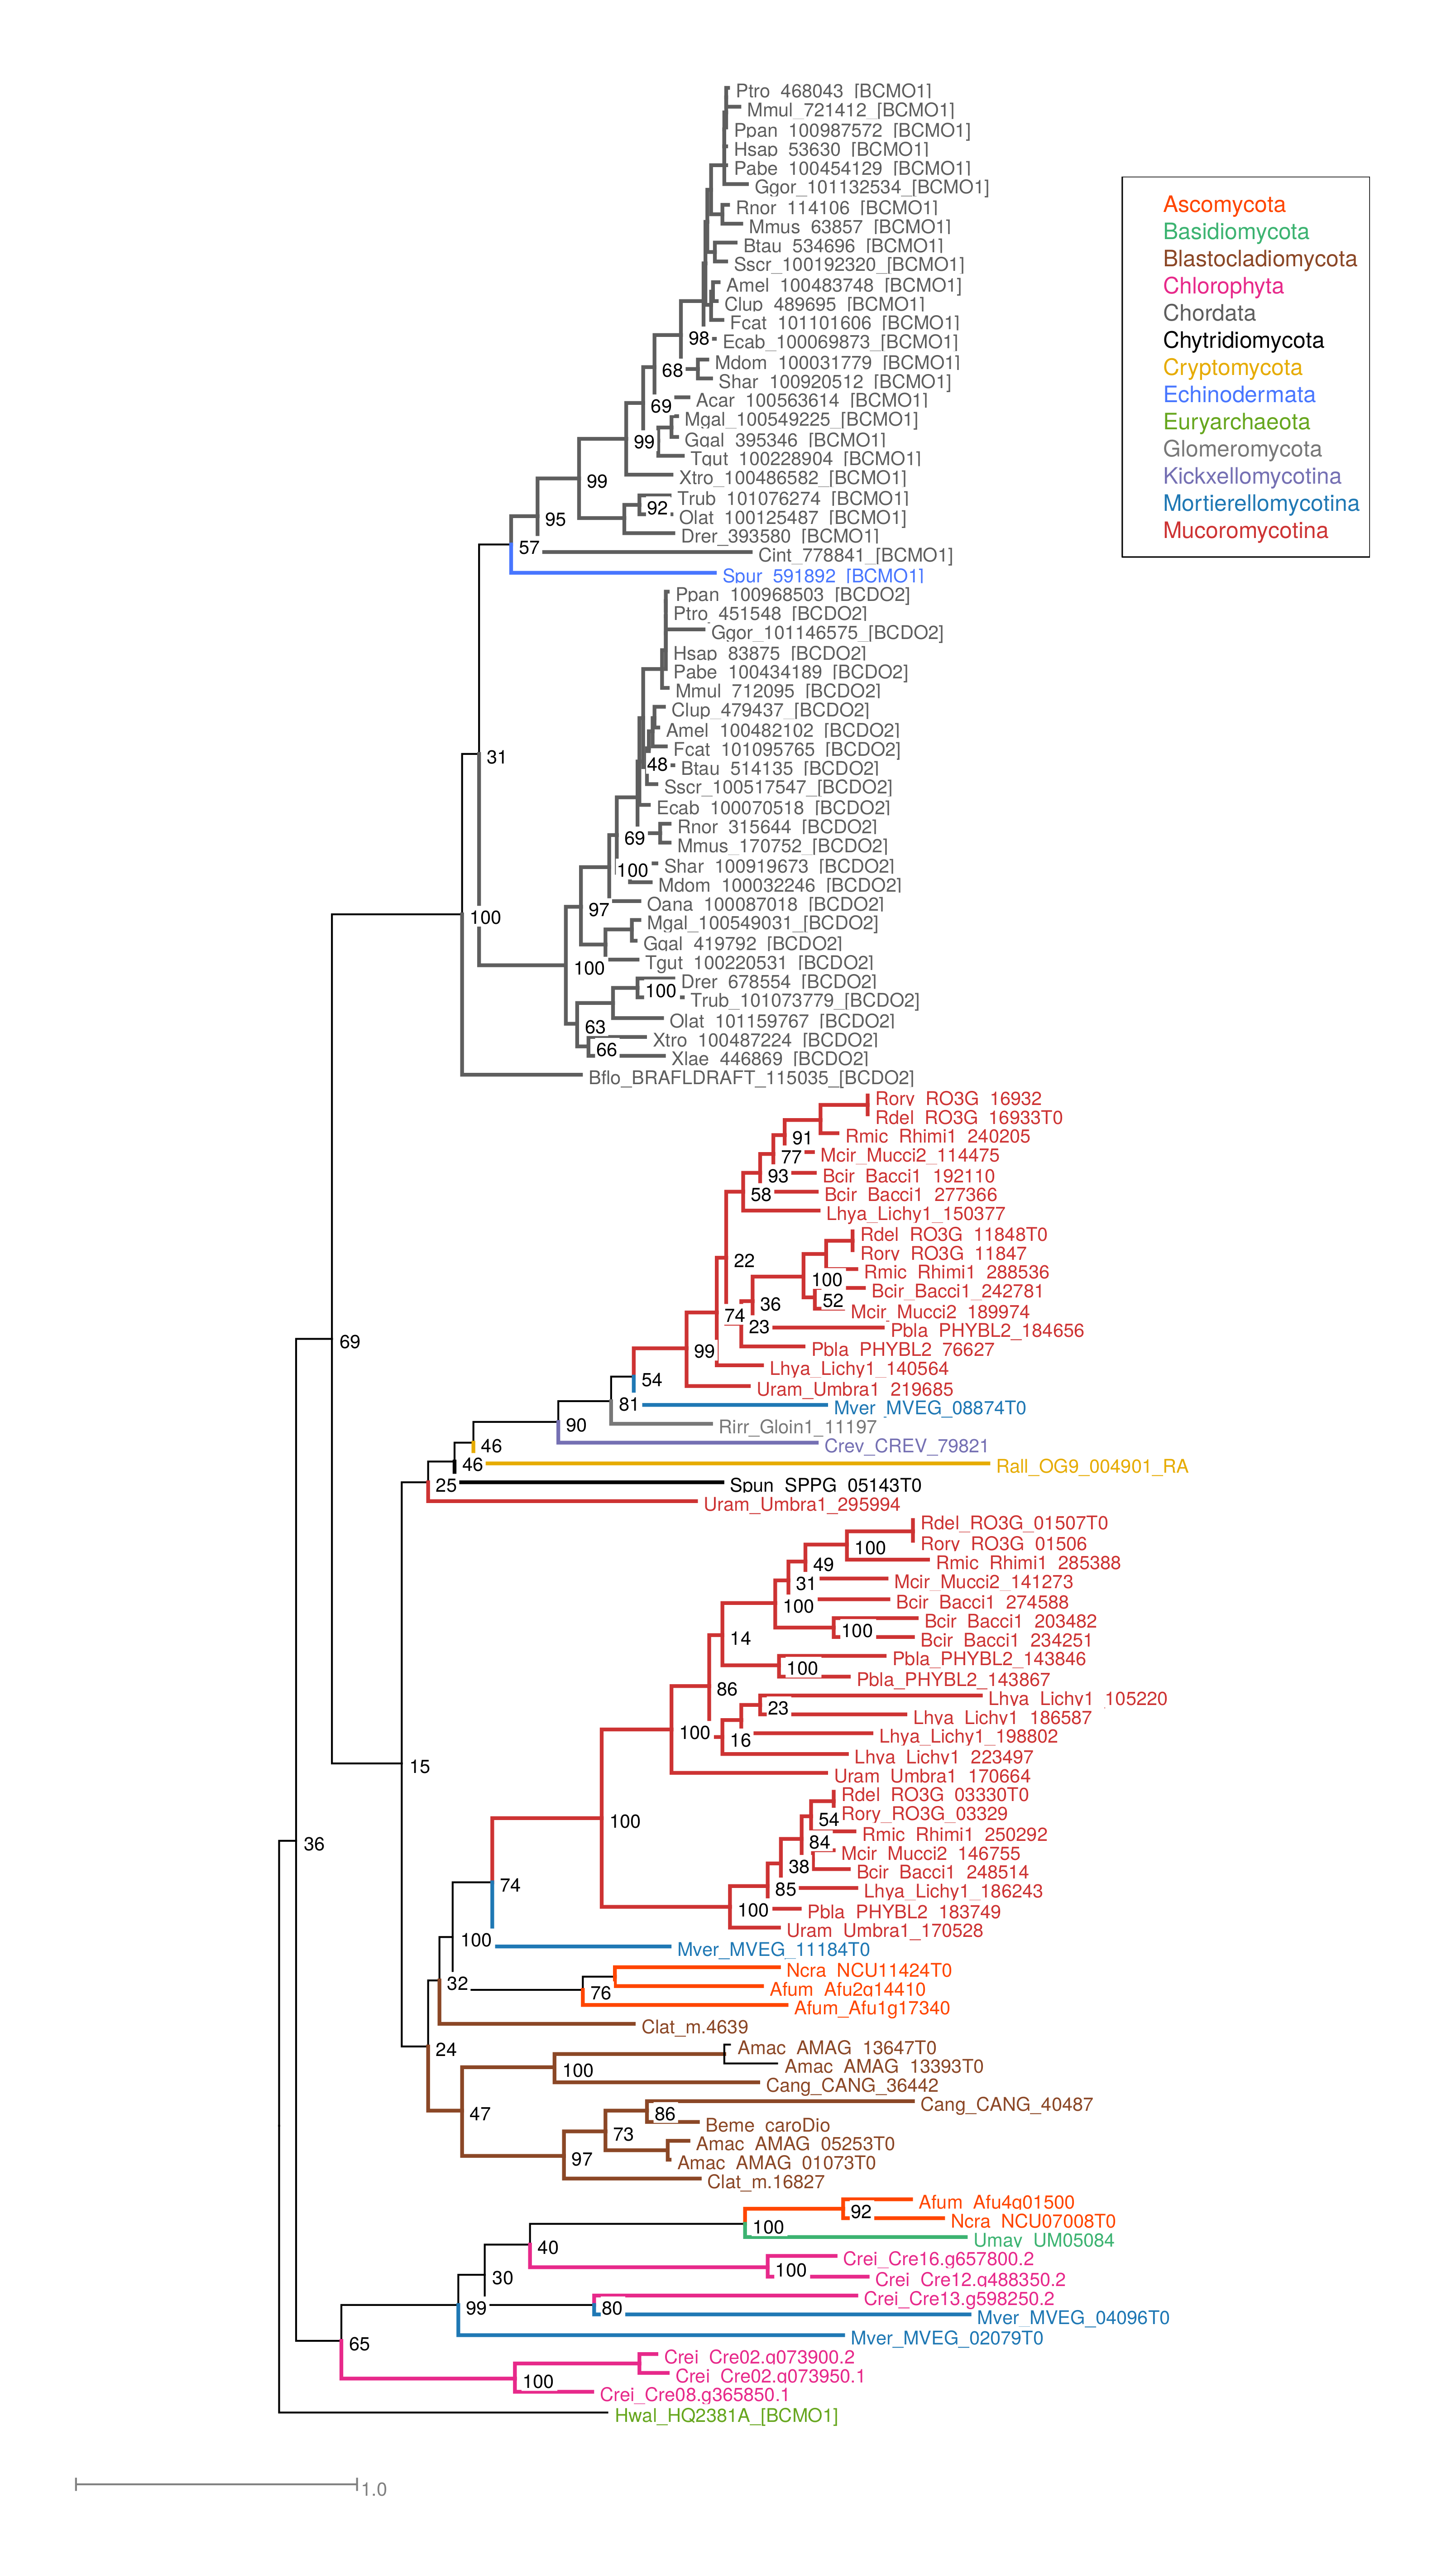
\includegraphics[width=4in]{./Chapter_Coelomomyces/img/BCMO1DO2.png}
  \caption[BCMO1 history]{Phylogenetic history of BCMO1 founds in Fungi and Metazoan lineages}
  \label{fig:ChClat_BCMO1DO2}
\end{figure}

% WC1 PAS alignment
\begin{figure}[tbp]
  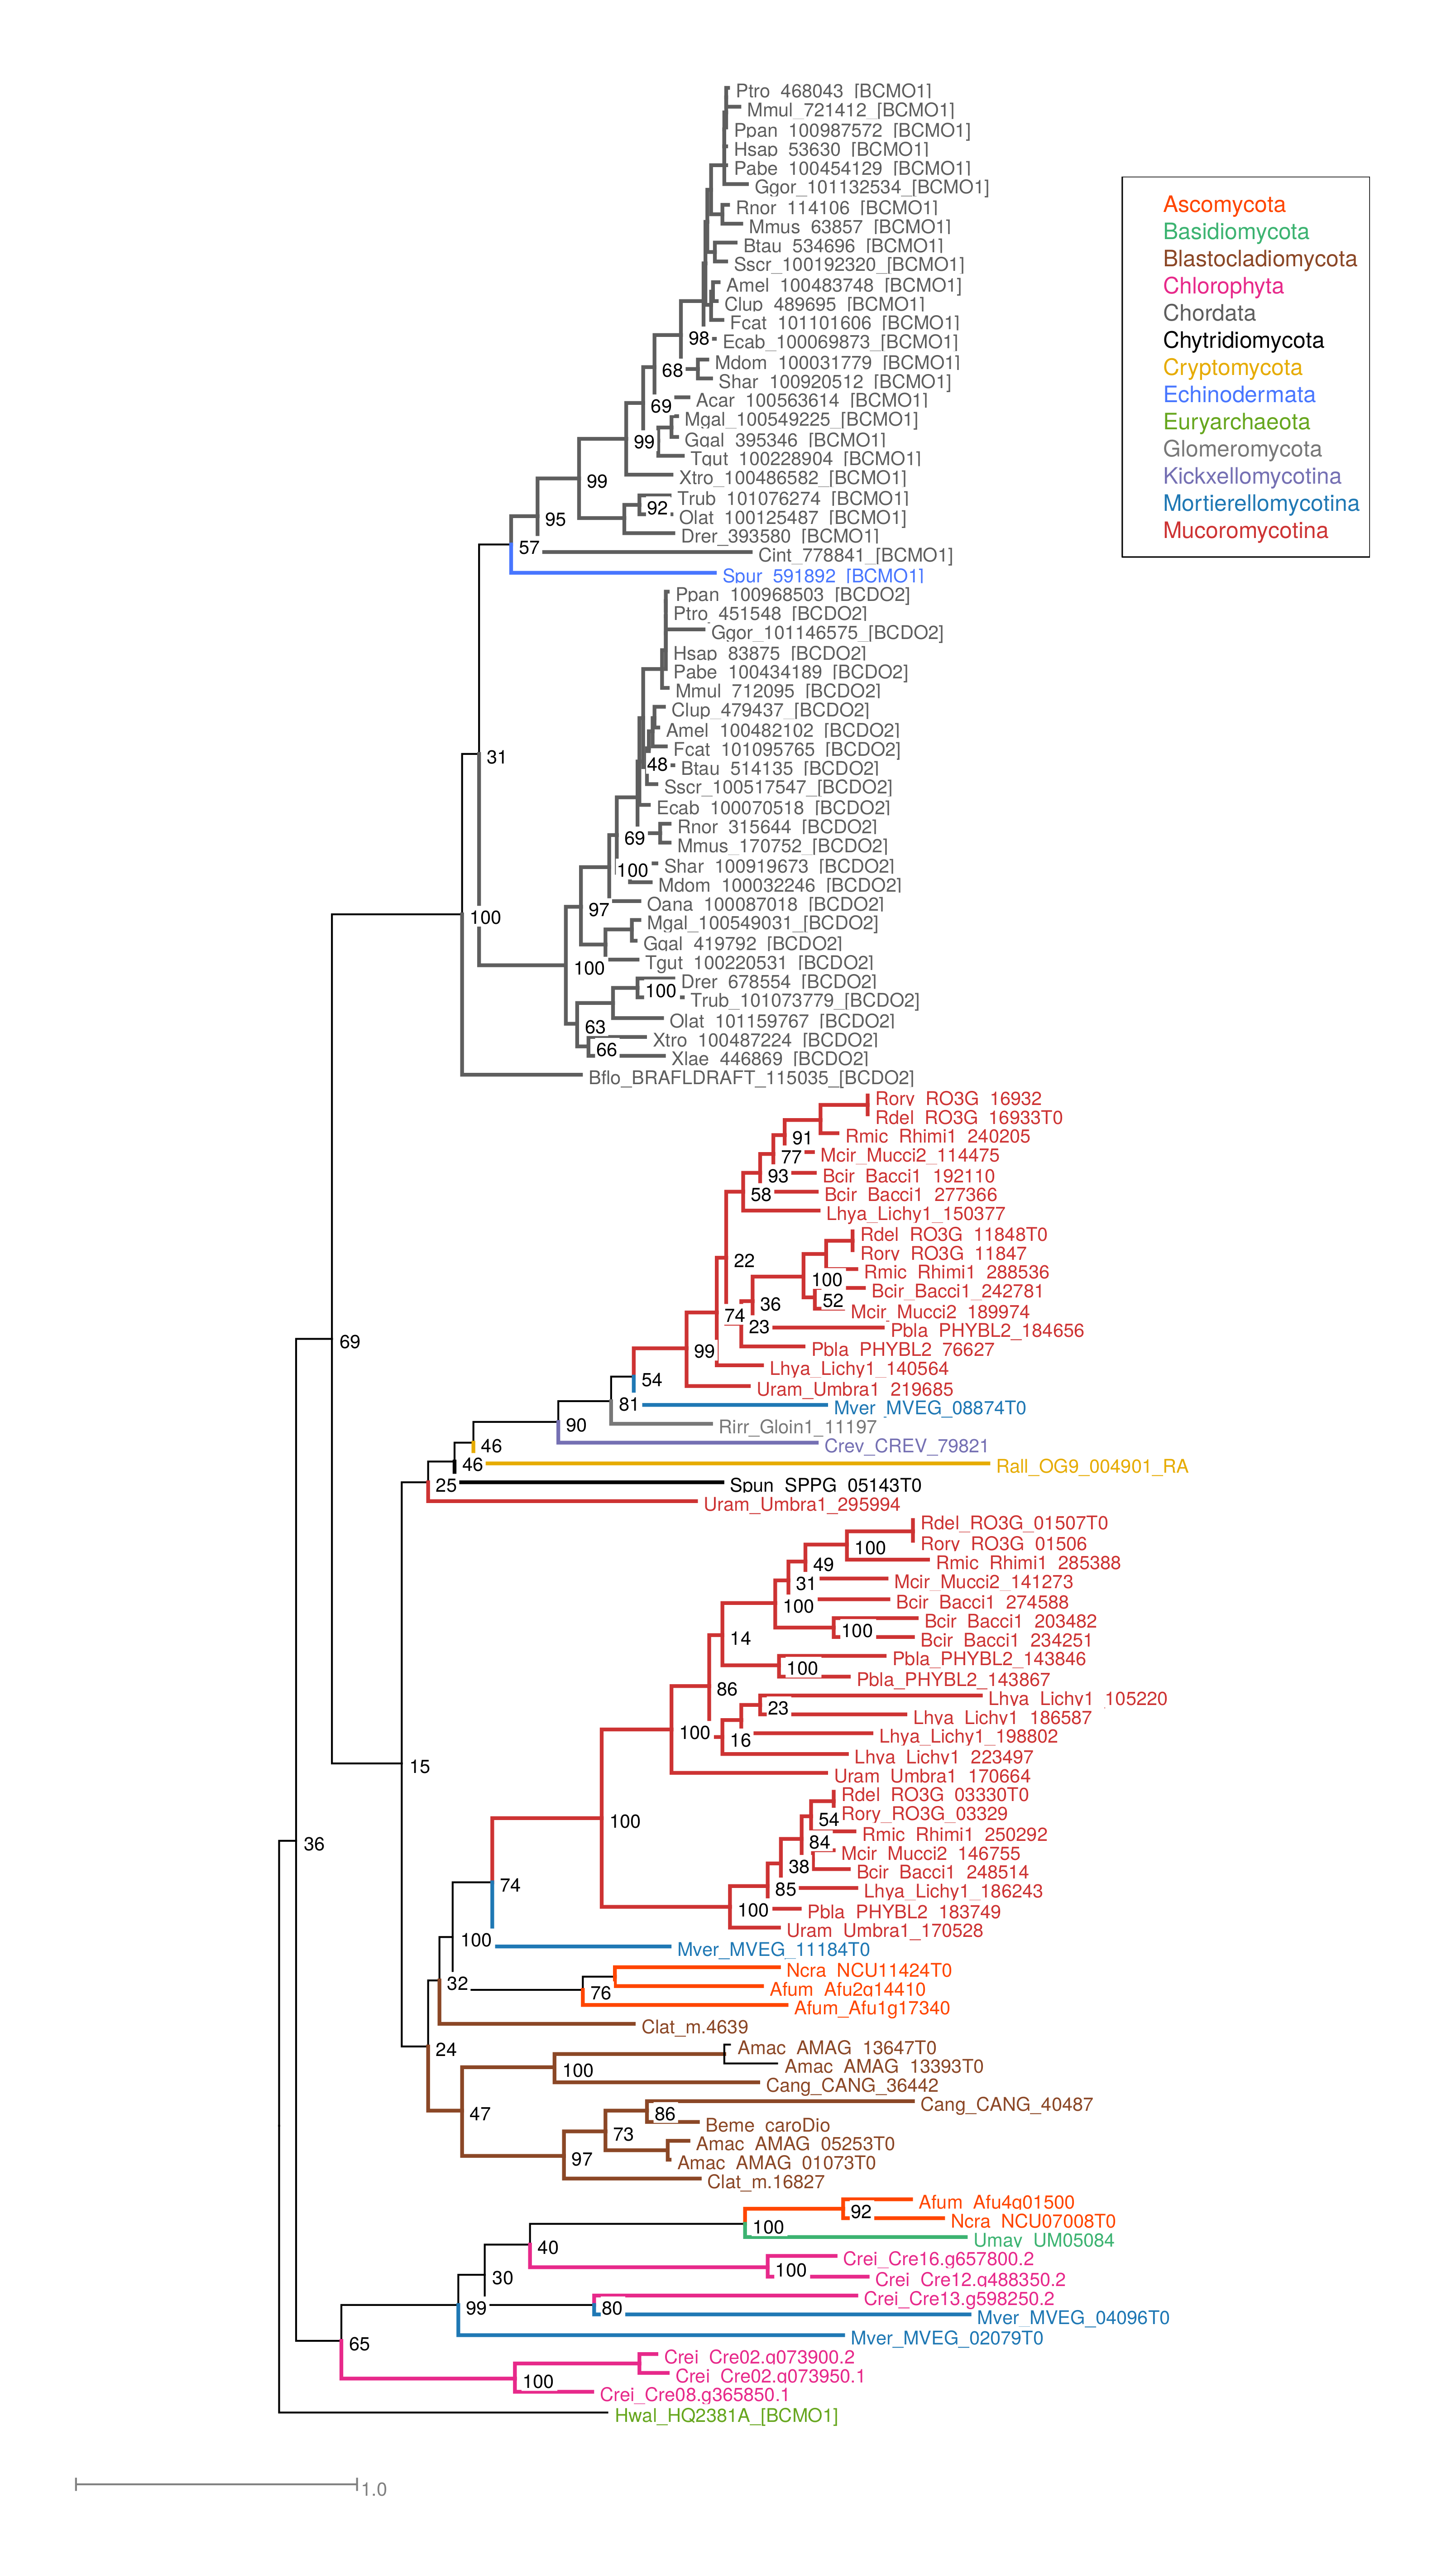
\includegraphics[width=4in]{./Chapter_Coelomomyces/img/BCMO1DO2.png}
%  \begin{texshade}{./Chapter_Coelomomyces/dat/PAS_alignment.fasta_aln}
%    \threshold[80]{50}
%    \shadingmode[allmatchspecial]{similar}
%    \setends{1}{5..300}
%    %\hideconsensus
%  \end{texshade}
  \caption[PAS alignment of WC1 homologs]{Multiple sequence alignment of PAS-domain in fungal WC1 homologs}
  \label{fig:ChClat_PASaln}
\end{figure}
